Spatial data and query processing have become ubiquitous due to proliferation of location-based services such as digital mapping, location-based social networking,
and geo-targeted advertising. Motivated by the performance benefits of learned indices
for one-dimensional data, this section explores the application of learned index for spatial data. The main motivation is to use machine learning models through several steps and generate a learned index for spatial data to reduce the storage consumption and IO cost compared to existing indexes such as R-Tree.

\subsubsection{Motivation}
In the last section, we described a recursive model index (RMI) that consists of a
number of machine learning models staged into a hierarchy to enable synthesis of specialised index structures, termed learned indexes. Provided with a search key x, RMI predicts the position of x's data with some error bound, by learning the cumulative distribution function (CDF) over the key search space. However, the idea of RMI is not applicable in the context of spatial data as spatial data invalidates the assumption required by RMI that the data is sorted by key and that any imprecision can be easily corrected by a localised search. Although it is possible to learn multi-dimensional CDFs, such CDFs will result in searching local regions qualified on one dimension but not all dimensions.

For example, consider the joint cumulative function of two random variables X and Y defined as $F_{XY}(x, y)=P(X\leq x, Y\leq y)$.

The joint CDF satisfies the following properties:

\begin{itemize}
  \item  {$F_X(x)=F_{XY}(x,\infty)$, for any x (marginal CDF of X)}
  \item  {$F_Y(y)=F_{XY}(\infty,y)$, for any y (marginal CDF of Y)}
  \item  {if $X$ and $Y$ are independent, then $F_{XY}(x,y)=F_X(x)F_Y(y)$}
\end{itemize}

\textcolor{blue} {Need to find a solid argument to explain why learning multi dimensional CDFs will result in  searching local regions qualified on one dimension. }
LISA solves this problem by partitioning search space into a series of grid cells based on the data distribution and building a partially monotonic function according to the borders of cells to map the data from $\mathbb{R}^d$ into $\mathbb{R}$.


\subsubsection{Baseline Method}  

We can extend the learned index method for range queries on spatial data by using a mapping function. This baseline method works as follows. We first sort all keys according to their mapped values and divide the mapped values into equal number of cells. If a point
(x,y)’s mapped value is larger than those of the keys stored
in the first i cells, i.e. $M(x,y) > \sup \bigcup\limits_{j=0}^{i-1} M(C_{j})$, we store (x,y) in cell i. Subsequently, for a query rectangle
qr = $[l_{0},u_{0}) \times [l_{1},u_{1})$, we only need to predict $i_{1}$ and $i_{2}$, the indices of $(l_{0}, l_{1})$ and $(u_{0},u_{1})$, respectively, scan the keys in $i_{2}$ - $i_{1}$ + 1 cells, and those keys that fall in the query rectangle qr . 

\subsubsection{Definitions}

This section presents the definition

\begin{enumerate}
	\item \textbf{Key}. A key k is a unique identifier for a data record with $k = (x_{0}, x_{1}) \in \mathbb{R}^{2}$. 
    %\textcolor{blue} {Need to check how to write d-1 in subscript }
    
	\item \textbf{Cell}. A grid cell is a rectangle whose lower and upper corners are points $(l_{0},l_{1}) and  (u_{0},u_{1})$, i.e.,  cell = $(l_{0},u_{0}) \times [l_{1},u_{1})$
	
	\item \textbf{Mapping Function}. A mapping function M is a partially monotonic function on the domain $\mathbb{R}^{2}$ to the non-negative range,i.e $M:[0,X_{0}]\times[0,X_{1}]\to [0,+\infty)$ such that $M(x_{0},x_{1}) \leq M(y_{0},y_{1})$ when $x_{0} \leq y_{0}$ and $x_{1} \leq y_{1} $
    
\end{enumerate}
% $f:\mathbb{R}\to\mathbb{R}, x\to y$ where $x$ is the input index and $y$ is the corresponding page block


\subsubsection{Training}

In order to construct the baseline model, we need to have several parameters listed below:
\begin{enumerate}
	\item The training dataset, notated as $(X, Y)$ with entries notated as $(x,y)$. $X$ represents the two dimensional key values, and $Y$ represents the corresponding data item value. 
	\item This number represents the number of cells(pages) into which the key space mapped values will be divided. It is an integer variable. Pages or cells will be used interchangeably in the next section to represents the subset of keys in a particular cell. 
\end{enumerate}

During training, sort all keys according to their mapped values, divide the keys into equal sized cells(pages), and store the mapped values of first and last key for each page into an array. For prediction, find the page corresponding to mapped value of query point, and scan this page sequentially. 
%The training algorithm is shown in f. There will be only one root model that receives the whole training data. After the root model is trained, we iterate over all the training data and predict the page by the root model. After the iteration, we get a new set of pairs $(X, Y_0)$. Then we map $\forall y_0\in Y_0$ into the selected model id in next stage by $\texttt{next}=y_0 * N_M^{(i+1)}/\texttt{max(Y)}$.

\begin{algorithm}[H]
    \SetAlgoLined
    \SetKwInOut{Input}{input}
    %\Input{\texttt{num\_of\_stages; num\_of\_models; types\_of\_models; x; y}}
     \Input{\texttt{num\_of\_cells;x;y}}
      \texttt{trainset=[$(x,y);x \in \mathbb{R}^{2};y \in \mathbb{R}$]} \\
     \For{$i\gets0$ \KwTo $len(x)$}{
            	\texttt{x[i].mapped\_value = x[i][0]+x[i][1]} \\
            
     }
     \texttt{Sort x based on x.mapped\_value}\\
     \texttt{Divide x into equal size pages according to num\_of\_cells}\\
     \texttt{Store mapped value of first and last key for each page }\\
      \For{$i\gets0$ \KwTo num\_of\_cells} %\Comment{Store mapped value of first and last key for each page}
     {
         \texttt{denseArray[i].lower = first key in page i  } \\
		 \texttt{denseArray[i].upper = last key in page i  }
		
     }
     \caption{Training Algorithm for Lisa Baseline Method}
     \label{Training_Lisa_Baseline}
\end{algorithm}

\subsubsection{Prediction}

\begin{algorithm}[H]
    \SetAlgoLined
    \SetKwInOut{Input}{input}
    \Input{\texttt{x\_test: Key Value to be searched }}
    \texttt{x\_test.mapped\_value = x\_test[0]+x\_test[1] } \\
    \For{$i\gets0$ \KwTo $len(denseArray)$}
    {
        \uIf{$((x\_test.mapped\_value \geq denseArray[i].lower) \& (x\_test.mapped\_value \leq denseArray[i].upper))$} 
        {
		    \texttt{Key is in Page i } \\
		    \texttt{break }
		}
    }
  
 	 \texttt{Sequentially search for x\_test in page j} \\
     \caption{Prediction Algorithm for Lisa Baseline Model }
\end{algorithm}

\subsubsection{Limitation}
Prediction cost in baseline method consists of following two parts.
%search cost for the page which contains the key, and once the page is found, scan cost of all the keys in the page to match the query point. If page size is small, first cost will be high as keys will be divided into larger number of pages. On the other hand, if page size is large, number of pages will be smaller, number of keys per page will be higher, resulting in higher cost of sequential scan with in the page.

\begin{enumerate}
	\item Search cost for the page which contains the key. If page size is small, this cost will be high as keys will be divided into larger number of pages
	\item Scan cost of all the keys in a particular page to match the query point. If page size is large, number of pages will be smaller, number of keys per page will be higher, resulting in higher cost of sequential scan with in the page. 
\end{enumerate}
Consider the example in figure \ref{fig:BaseLine_Method_Limitation}. Dataset is divided into 3 sections based on the mapped values. Any point or range query in the second triangle(page) will result into a sequential scan through all 14 keys in the triangle.   

\begin{figure*}[t]
    \centering
    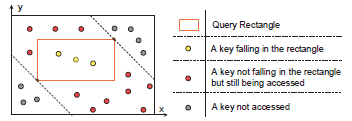
\includegraphics[width=0.9\textwidth]{graphs/Lisa_Baseline_Model_Limitation.png}
    \caption{Baseline Method Limitation }
    \label{fig:BaseLine_Method_Limitation}
\end{figure*}

\subsubsection{Lisa Overview}
Given a spatial dataset, we generate the mapping function
M, the shard prediction function SP and a series of local
models. Based on them, we build our index structure, LISA, to
process range query,KNN query and data updates. LISA consists of four parts: the representation of grid cells, the mapping function M, the shard prediction function SP, and the local models for all shards. As illustrated in the figure. the procedure of building LISA is composed of four parts.

\begin{figure*}[t]
    \centering
    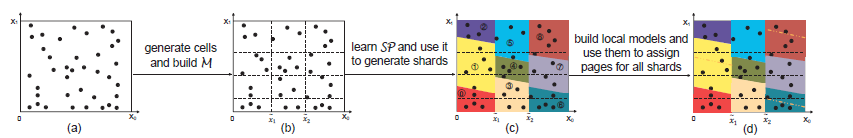
\includegraphics[width=17cm,height=4cm]{graphs/Lisa_Overview.png}
    \caption{Lisa Framework }
    \label{fig:Lisa_Framework}
\end{figure*}

This section presents the additional definition for Lisa model.  

\begin{enumerate}
	\item \textbf{Shard}.shard S is the preimage of an
interval $[a, b) \subseteq [0, +1)$ under the mapping function M,  i.e., $S = M^{-1}([a.b))$.
    
	\item \textbf{Local Model}. local model $L_{i}$ is a model
that processes operations within a shard Si . It keeps dynamic
structures such as the addresses of pages contained by $S_{i}$ .
\textcolor{blue} {Will add further details as we start working on corresponding modules.}	
\end{enumerate}


\subsubsection{Lisa Design}
\textbf{Grid Cells Generation} 
First task in Lisa implementation is to partition the 2 dimensional key space into a series of grid cells based on the data distribution
along a sequence of axes and numbering the cells also along
these axes. The principal idea behind this partition strategy is to divide the key space into cell boundaries and apply a mapping function to create monotonically increasing mapping values at the cell boundaries, i.e. mapped value of all keys in cell i will be less than mapped values of keys in cell j, if i <j. Consider the example shown in the figure \ref{fig:Cell_Parttion} total number of keys are 18, and we decided to partition the key space into 9 cells, resulting in 2 keys per cell. To partition the key space, we first sort the keys values according to $1^{st}$  dimension, divide the keys into 3 cells each containing 6 keys. Then for each cell, we sort the keys again according to $2^{nd}$  dimension, and divide the keys in each cell into 3 new cells. 


\begin{figure*}[t]
    \centering
    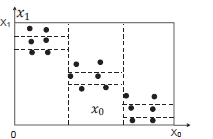
\includegraphics[width=0.8\textwidth]{graphs/Cell_partition.png}
    \caption{Cell Partition Strategy }
    \label{fig:Cell_Parttion}
\end{figure*}


\begin{algorithm}[H]
    \SetAlgoLined
    \SetKwInOut{Input}{input}
    %\Input{\texttt{num\_of\_stages; num\_of\_models; types\_of\_models; x; y}}
     \Input{\texttt{num\_of\_cells;x; y}}
     \texttt{trainset=[$(x,y);x \in \mathbb{R}^{2};y \in \mathbb{R}$]} \\
     \texttt{$keysPerPage =  len(x) / num\_of\_cells $}\\
     \texttt{Sort x based on first dimension x[:][0]]}\\
     \texttt{In first for loop, divide the keys into equal size subsets based on first dimension }\\
     \For{$i\gets0$ \KwTo $\sqrt(num\_of\_cells)$}  
     {
        \texttt{Store the 1st dimensional coordinates of first and last key for each cell.Each such cell will contain $keysPerPage*sqrt(num\_of\_cells)$ keys } \\
        %\texttt{$cellMatrix[i].lower\_x0 = 1st dimensional coordinates$ of first key in the cell  } \\
		%\texttt{$cellMatrix[i].upper\_x0 = 1st dimensional coordinates$ of last key in the cell  }
		
     }
     %\texttt{After first for loop, each cell in sqrt(num\_of\_cells) will contain $keysPerPage*sqrt(num\_of\_cells)$ keys }\\
     
     \texttt{Sort keys in each cell based on 2nd dimension,x[:][1] }\\
     
      \For{$i\gets0$ \KwTo $\sqrt(num\_of\_cells)$} %\Comment{Store mapped value of first and last key for each page}
      {
         \For{$j\gets0$ \KwTo $\sqrt(num\_of\_cells)$}
         {
            \texttt{Store the 2nd dimensional coordinates of first and last key for each cell.} \\
            %\texttt{$cellMatrix[i].lower_x0 = 2nd dimensional coordinates$ of first key in the cell  } \\
	    	%\texttt{$cellMatrix[i].upper_x0 =  2nd dimensional Coordinates$ of last key in the cell}
		 }
      }
     \caption{Grid Cell Generation Algorithm for Lisa Method}
     \label{Training_Lisa_Baseline}
\end{algorithm}






